\chapter{The Klessydra DSP Accelerator and its Modular Re-engineering}
\label{ch:architecture}

This chapter describes the vector accelerator that is the subject of the thesis
and the structural re-engineering that makes the rest of the work possible.
Section~\ref{sec:arch-overview} gives an overview of the accelerator and its
place in the Klessydra core. Section~\ref{sec:arch-datapath} walks through the
datapath and its functional units. Section~\ref{sec:arch-mapping} describes the
mapping and control layers and the replication mechanism.
Section~\ref{sec:arch-breakdown} explains the modular ``break-down'' of the
original monolithic design and why it is a prerequisite for selective hardening.

\section{Overview of the accelerator}
\label{sec:arch-overview}

The Klessydra DSP unit is a SIMD vector coprocessor attached to the Klessydra
RISC-V core. It executes custom vector instructions --- vector add, multiply,
shift, compare, and multiply-accumulate among them --- on operands held in a
dedicated scratchpad memory (SPM). The accelerator is deeply parameterised
through VHDL generics and package constants; the parameters most relevant to
this work are summarised in Table~\ref{tab:params}.

\begin{table}[htbp]
\centering
\caption{Principal configuration parameters of the Klessydra DSP accelerator,
with the values used as the experimental baseline in this thesis.}
\label{tab:params}
\small
\begin{tabular}{lp{8.2cm}c}
\toprule
Parameter & Meaning & Baseline value \\
\midrule
\texttt{Data\_Width}      & Scalar element width in bits                              & 32 \\
\texttt{SIMD}             & Number of SIMD sub-lanes per accelerator lane             & 2 \\
\texttt{SIMD\_Width}      & Aggregate datapath width (\texttt{SIMD}$\times$32) in bits & 64 \\
\texttt{ACCL\_NUM}        & Number of parallel accelerator lanes                      & 1 / 3 \\
\texttt{FU\_NUM}          & Number of functional-unit sets                            & 1 / 3 \\
\texttt{THREAD\_POOL\_SIZE} & Number of interleaved hardware threads                  & 3 \\
\texttt{SPM\_NUM}         & Number of scratchpad banks                                & 4 \\
\texttt{replicate\_accl\_en} & Enables the replicated multi-lane datapath             & 0 / 1 \\
\bottomrule
\end{tabular}
\end{table}

When \texttt{replicate\_accl\_en} is disabled, a single accelerator lane
(\texttt{ACCL\_NUM}~$=$~\texttt{FU\_NUM}~$=$~1) serves the thread pool; this is
the substrate for per-functional-unit hardening (Scenario~A in
Chapter~\ref{ch:framework}). When replication is enabled, three lanes are
instantiated (\texttt{ACCL\_NUM}~$=$~\texttt{FU\_NUM}~$=$~3), which is the
substrate for replication-based redundancy (Scenario~B).

\section{The datapath and its functional units}
\label{sec:arch-datapath}

The heart of the accelerator is its arithmetic datapath, organised as a set of
pipelined functional units (FUs) fed by an input mapping stage and drained by an
output mapping stage. Figure~\ref{fig:datapath} sketches the structure.

\begin{figure}[htbp]
\centering
\begin{tikzpicture}[
  node distance=6mm and 9mm,
  box/.style={draw, rounded corners, minimum height=8mm, minimum width=20mm, align=center, font=\footnotesize, fill=blue!5},
  fu/.style={draw, rounded corners, minimum height=8mm, minimum width=22mm, align=center, font=\footnotesize, fill=orange!12},
  io/.style={draw, minimum height=8mm, minimum width=18mm, align=center, font=\footnotesize, fill=gray!10},
  arr/.style={-{Latex[length=2mm]}, thick}
]
\node[io] (spm) {Scratchpad\\Memory (SPM)};
\node[box, right=of spm] (inmap) {Input\\Mapping};
\node[fu, right=18mm of inmap, yshift=15mm] (add) {Adders};
\node[fu, below=4mm of add] (mul) {Multipliers};
\node[fu, below=4mm of mul] (shf) {Shifters};
\node[fu, below=4mm of shf] (cmp) {Comparators};
\node[fu, below=4mm of cmp] (acc) {Accumulator};
\node[box, right=18mm of mul] (outmap) {Output\\Mapping};
\node[io, right=of outmap] (spm2) {Scratchpad\\Memory (SPM)};
\node[box, above=10mm of inmap] (ctrl) {Pipeline Controller\\/ FU Handler};

\draw[arr] (spm) -- (inmap);
\foreach \f in {add,mul,shf,cmp,acc} \draw[arr] (inmap.east) -- (\f.west);
\foreach \f in {add,mul,shf,cmp,acc} \draw[arr] (\f.east) -- (outmap.west);
\draw[arr] (outmap) -- (spm2);
\draw[arr] (ctrl.south) -- (inmap.north);
\draw[arr, dashed] (ctrl.east) -| (outmap.north);
\begin{scope}[on background layer]
\node[draw, dashed, rounded corners, fit=(add)(mul)(shf)(cmp)(acc), inner sep=4mm, label={[font=\footnotesize\itshape]above:Functional Units}] {};
\end{scope}
\end{tikzpicture}
\caption{Block-level structure of the Klessydra DSP accelerator. Operands are
read from the scratchpad memory, distributed by the input mapping stage to the
functional units, and the results are gathered by the output mapping stage and
written back. The pipeline controller and FU handler sequence the units.}
\label{fig:datapath}
\end{figure}

\subsection{Vector adders}

The adder unit performs vector additions and subtractions and is configurable in
the way it propagates carries, so that one physical adder array can implement
byte-wise (\texttt{KADDV8}), half-word (\texttt{KADDV16}), or full-word
(\texttt{KADDV32}) additions by selectively breaking or passing the carry chain.
Internally it is pipelined across two stages (\texttt{DSP\_Adders\_stg\_1} and
\texttt{DSP\_Adders\_stg\_2}) with a synchronisation block
(\texttt{DSP\_Adders\_Sync}) that aligns results to the pipeline. The adder also
exports the most-significant-bit information used by the comparator unit.

\subsection{Vector multipliers}

The multiplier unit is the largest and most arithmetically complex functional
unit. It is built as a multi-stage pipeline
(\texttt{DSP\_Multipliers\_stg\_1}, a combinational partial-product stage
\texttt{DSP\_Multipliers\_stg\_1\_comb}, and \texttt{DSP\_Multipliers\_stg\_2})
so that the long multiplication critical path is broken into balanced pipeline
stages. Because of its size, the multiplier dominates the area cost of any
redundancy scheme that includes it --- a fact that the results in
Chapter~\ref{ch:results} make very visible.

\subsection{Vector shifters}

The shifter unit performs logical and arithmetic shifts across the vector lanes.
It comprises a combinational shift network (\texttt{DSP\_Shifters\_comb}) and two
pipeline stages (\texttt{DSP\_Shifters\_stg\_1}, \texttt{DSP\_Shifters\_stg\_2}).
Its area is modest and comparable to the adder.

\subsection{Vector comparators}

The comparator unit (\texttt{DSP\_Comparators\_Unit}) evaluates relational
operations across the vector elements, consuming the most-significant-bit
information exported by the adder. It is the smallest of the four arithmetic
functional units, which makes it the cheapest to protect.

\subsection{Accumulator}

The accumulation stage (\texttt{RTL-Accumulator}) implements the reduction
required by multiply-accumulate-style instructions, summing partial results
across iterations. In the present study the accumulator is treated as part of
the surrounding datapath rather than hardened individually, but the modular
structure would allow it to be wrapped just like the other units.

\section{Mapping, control, and replication}
\label{sec:arch-mapping}

\subsection{Mapping stages}

The \texttt{DSP\_Mapping} layer is responsible for routing operands from the
scratchpad to the functional units and routing results back. It exists in two
flavours --- a \emph{multithread} mapper
(\texttt{DSP\_Mapping\_IN\_Unit\_Multithread} and the matching out-mapper) and a
\emph{multicore} mapper (\texttt{DSP\_Mapping\_IN\_Unit\_Multicore} and
\texttt{DSP\_Mapping\_Multicore\_Out\_Mapper}). The multicore mapper is the one
exercised when the accelerator is replicated into multiple lanes, and, as
explained in Chapter~\ref{ch:framework}, it is also where replication-based
voting is inserted.

\subsection{Control: pipeline controller and FU handler}

Two control blocks sequence the datapath. The \texttt{DSP\_Pipeline\_Controller}
generates the stage-enable and halt signals that advance operands through the
functional-unit pipelines. The \texttt{DSP\_FU\_Handler} --- with dedicated
multicore (\texttt{MC}) and multithread (\texttt{MT}) variants and an enabler
synchroniser (\texttt{DSP\_FU\_Enabler\_Sync}) --- arbitrates which functional
unit is active for which thread or lane at any cycle, enabling the interleaved
multithreading that is characteristic of Klessydra. An exception-control unit
(\texttt{DSP\_Excpt\_Cntrl\_unit}) handles state recovery.

\subsection{Replication}

The top-level \texttt{replicate\_accl\_en} generic switches the accelerator
between a single-lane and a three-lane configuration. In the replicated
configuration three complete accelerator lanes operate in parallel, multiplying
throughput. This replicated datapath is significant for reliability because the
expensive functional-unit copies it instantiates can be \emph{reused} for
redundancy: rather than building new replicas, the redundancy logic simply
compares or votes the results that the lanes already produce. The cost of doing
so is quantified in Chapter~\ref{ch:results}.

\section{The modular break-down}
\label{sec:arch-breakdown}

\subsection{From monolith to hierarchy}

In its original form, much of the accelerator's arithmetic was expressed as a
single, tightly interwoven block. While this is acceptable for a fixed design,
it is hostile to reliability engineering: there is no entity boundary at which a
redundancy wrapper can be attached to one functional unit without entangling it
with the others, and there is no clean place to insert instrumentation. The
first engineering task of this thesis was therefore to \emph{break down} the
accelerator into the clean hierarchy summarised in Figure~\ref{fig:hierarchy}.

\begin{figure}[htbp]
\centering
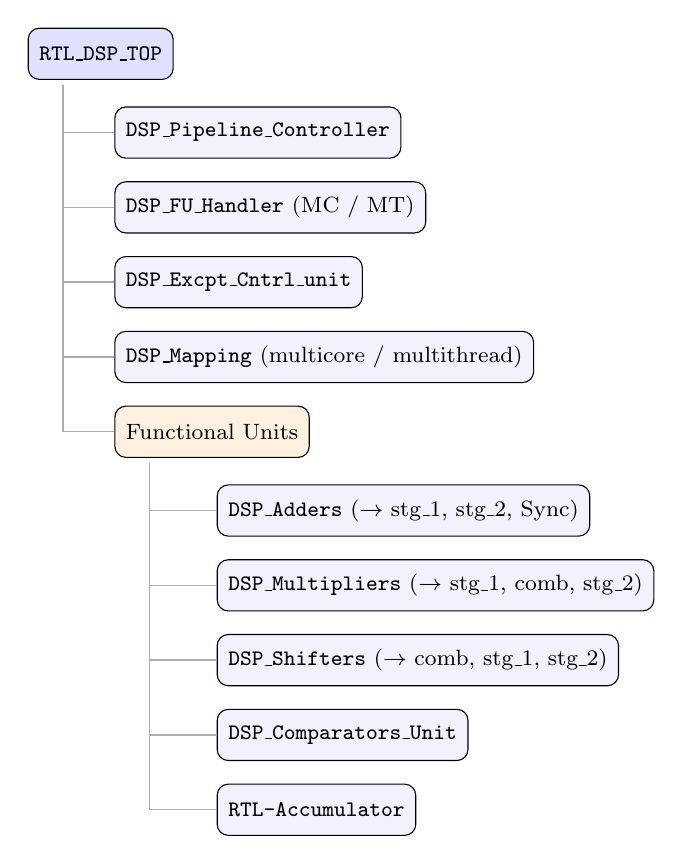
\begin{tikzpicture}[
  comp/.style={draw, rounded corners, fill=blue!5, inner sep=4pt, anchor=west,
               font=\footnotesize, minimum height=6.5mm},
  topb/.style={comp, fill=blue!12},
  fub/.style={comp, fill=orange!12},
  bus/.style={draw, gray!65, line width=0.5pt}
]
% --- level 0 ---
\node[topb] (top) at (0,0) {\texttt{RTL\_DSP\_TOP}};
% --- level 1 (children of TOP) ---
\node[comp] (pc) at (1.1,-1.00) {\texttt{DSP\_Pipeline\_Controller}};
\node[comp] (fh) at (1.1,-1.95) {\texttt{DSP\_FU\_Handler} (MC / MT)};
\node[comp] (ex) at (1.1,-2.90) {\texttt{DSP\_Excpt\_Cntrl\_unit}};
\node[comp] (mp) at (1.1,-3.85) {\texttt{DSP\_Mapping} (multicore / multithread)};
\node[fub]  (fu) at (1.1,-4.80) {Functional Units};
% --- level 2 (children of Functional Units) ---
\node[comp] (add) at (2.4,-5.80) {\texttt{DSP\_Adders} ($\rightarrow$ stg\_1, stg\_2, Sync)};
\node[comp] (mul) at (2.4,-6.75) {\texttt{DSP\_Multipliers} ($\rightarrow$ stg\_1, comb, stg\_2)};
\node[comp] (shf) at (2.4,-7.70) {\texttt{DSP\_Shifters} ($\rightarrow$ comb, stg\_1, stg\_2)};
\node[comp] (cmp) at (2.4,-8.65) {\texttt{DSP\_Comparators\_Unit}};
\node[comp] (acc) at (2.4,-9.60) {\texttt{RTL-Accumulator}};
% --- connectors: level-1 bus drops from TOP, elbows into each child ---
\draw[bus] (0.45,-0.40) -- (0.45,-4.80);
\foreach \y in {-1.00,-1.95,-2.90,-3.85,-4.80}{ \draw[bus] (0.45,\y) -- (1.10,\y); }
% --- connectors: level-2 bus drops from Functional Units ---
\draw[bus] (1.55,-5.20) -- (1.55,-9.60);
\foreach \y in {-5.80,-6.75,-7.70,-8.65,-9.60}{ \draw[bus] (1.55,\y) -- (2.40,\y); }
\end{tikzpicture}
\caption{Re-engineered module hierarchy of the accelerator. Each functional unit
is a self-contained VHDL entity with an explicit interface, exposing a clean
boundary at which redundancy wrappers and sensors can be attached.}
\label{fig:hierarchy}
\end{figure}

\subsection{Why isolation matters}

The decisive property of the re-engineered design is that each functional unit
is an independently instantiable entity with a fully specified port interface.
This has three consequences that the rest of the thesis depends on:

\begin{enumerate}
  \item \textbf{Selective hardening.} A redundancy wrapper can instantiate
        \emph{exactly one} functional unit two or three times and combine the
        copies, without touching any other unit. This is what makes
        per-functional-unit DMR and TMR possible.
  \item \textbf{Composability.} Because the wrappers preserve the original port
        interface, a hardened unit is a drop-in replacement for its unhardened
        counterpart; hardening any subset of units --- or all of them --- is
        simply a matter of choosing which wrappers to instantiate, controlled by
        the top-level \texttt{*\_DMR\_EN} / \texttt{*\_TMR\_EN} constants.
  \item \textbf{Instrumentability.} The same clean boundaries give the IJTAG
        sensor-insertion tool of Chapter~\ref{ch:ijtag} well-defined points at
        which to attach activity and thermal monitors.
\end{enumerate}

The modular hierarchy is thus not merely a tidy refactoring: it is the
enabling substrate for the fault-tolerance framework and the monitoring framework
that follow.
